\documentclass[runningheads]{llncs}
%
\usepackage[T1]{fontenc}
\usepackage{graphicx}
\usepackage{booktabs}
\usepackage{amsmath,amssymb}
\usepackage{array}
\usepackage{xcolor}
\usepackage[font=small,skip=4pt]{caption}
\usepackage{microtype}
\usepackage{flafter} % a float never appears before the text that introduces it
\usepackage{needspace}
\usepackage{placeins} % \FloatBarrier keeps floats inside their subsection
\usepackage{hyperref}
\renewcommand\UrlFont{\color{blue}\rmfamily}
\hypersetup{colorlinks=true,linkcolor=black,citecolor=black,urlcolor=blue}
% keep floats close to the text that references them
\renewcommand{\topfraction}{0.95}
\renewcommand{\bottomfraction}{0.9}
\renewcommand{\textfraction}{0.05}
\renewcommand{\floatpagefraction}{0.9}
\setlength{\textfloatsep}{10pt plus 2pt minus 2pt}
\setlength{\floatsep}{8pt plus 2pt minus 2pt}
\setcounter{topnumber}{3}
\setcounter{totalnumber}{4}
\raggedbottom % do not stretch vertical space on pages that end before a float page
%
\begin{document}
%
\title{Comparing Back-Propagation Optimizers for a Fully Connected Neural Network on a Five-Class MNIST Subset}
\titlerunning{Comparing Back-Propagation Optimizers for FCNNs}
%
\author{Nimitt Jain \and Dattaraj Saudagar \and Onkar Mulje}
\authorrunning{N. Jain, D. Saudagar, O. Mulje (Group 12)}
\institute{Group 12, CS601T: Deep Learning, Programming Assignment 3\\ August--November 2026 Semester}
%
\maketitle
%
\begin{abstract}
We train six fully connected neural networks on a five-class subset of MNIST (digits 0, 1, 2, 3
and 7): a wide and a narrow network for each depth of three, four and five hidden layers. Each is
trained with seven optimizers for back-propagation: stochastic gradient descent, batch gradient
descent, momentum (generalised delta rule), Nesterov accelerated gradient, AdaGrad, RMSProp and Adam.
For a fair comparison, the network, back-propagation and all update rules were implemented from
scratch exactly as in the course material. Every optimizer starts from the same initial weights of
its architecture, and training stops when the average training error of successive epochs changes by
less than $10^{-4}$. All 42 runs converged under this criterion. Pattern-mode optimizers with
momentum need only 7--27 epochs, whereas vanilla batch gradient descent with learning rate 0.001 needs
2038--2683 epochs and reaches only about 94\% accuracy. AdaGrad and RMSProp speed up batch-mode
training by factors of 4 to 46 but stop at a higher training error. Adam reaches the lowest errors
but is noisy with a batch size of one, and its stability depends strongly on where $\varepsilon$
enters the update. Its validation error rises while its training error keeps falling. Wide networks
are slightly more accurate than narrow ones, while depth has little effect. The best model, the wide
four-hidden-layer network trained with Nesterov accelerated gradient, achieves 99.26\% validation and
98.58\% test accuracy.
\keywords{Fully connected neural network \and Back-propagation \and SGD \and Momentum \and NAG \and AdaGrad \and RMSProp \and Adam}
\end{abstract}

\section{Introduction}
The goal of this assignment is to study how the choice of optimizer affects the training of a
fully connected neural network (FCNN) with back-propagation. Six FCNNs are trained, a wide and a
narrow network for each depth of three, four and five hidden layers. Each is trained with seven
optimizers: stochastic gradient descent (SGD), batch
(vanilla) gradient descent, SGD with momentum (generalised delta rule, GDR), Nesterov accelerated
gradient (NAG), AdaGrad, RMSProp and Adam. For every architecture we compare the number of epochs
needed for convergence, the training- and validation-error curves and the training/validation
accuracy. The architecture--optimizer pair with the highest validation accuracy is then evaluated on
the test set.

\section{Dataset and Pre-processing}
Group~12 was given a subset of MNIST with the five digit classes $\{0,1,2,3,7\}$. The data are
already split and perfectly balanced: 2277 training, 759 validation and 759 test images per class,
i.e.\ $N=11385$ training, 3795 validation and 3795 test images. Each $28\times28$ grey-scale
image is flattened into a 784-dimensional vector and its intensities are scaled to $[0,1]$
(division by 255). No other pre-processing or augmentation is used. The five classes are
encoded as indices $0,\dots,4$ and as one-hot target vectors.

\section{Methodology}
\subsection{Network Architectures}
All networks have 784 input units, ReLU hidden units and a softmax output layer with five units.
Table~\ref{tab:arch} lists the six architectures, which vary both depth and the number of nodes in
each layer. For each depth (3, 4 and 5 hidden layers) there is one \emph{wide} network (A1, A2, A3)
and one \emph{narrow} network (A4, A5, A6). Within every network the number of nodes decreases
towards the output layer. The wide networks have 111k--244k parameters and the narrow ones
53k--57k, dominated by the $784\times n_1$ weights of the first hidden layer. This design separates
the effect of depth (compare A1/A2/A3 or A4/A5/A6) from the effect of width (compare A1/A4, A2/A5
and A3/A6).
\begin{table}[!htb]
\centering
\caption{FCNN architectures (input 784, output 5, ReLU hidden layers, softmax output). A1--A3 are
wide and A4--A6 narrow networks with 3, 4 and 5 hidden layers.}\label{tab:arch}
\setlength{\tabcolsep}{9pt}
\begin{tabular}{llcr}
\toprule
Name & Layer sizes & Hidden layers & Parameters \\
\midrule
A1 & 784--128--64--32--5 & 3 & 110\,981 \\
A2 & 784--256--128--64--32--5 & 4 & 244\,357 \\
A3 & 784--128--96--64--48--32--5 & 5 & 123\,925 \\
A4 & 784--64--32--16--5 & 3 & 52\,933 \\
A5 & 784--64--64--32--16--5 & 4 & 57\,093 \\
A6 & 784--64--48--32--24--16--5 & 5 & 56\,205 \\
\bottomrule
\end{tabular}

\end{table}

\subsection{Forward Computation, Error and Back-Propagation}
The notation follows the course slides on FCNNs for classification with cross-entropy loss. The
training data are $\mathcal{D}=\{\mathbf{x}_n,\mathbf{y}_n\}_{n=1}^{N}$ with
$\mathbf{x}_n\in\mathbb{R}^{d}$, $d=784$, and the desired output
$\mathbf{y}_n=[y_{n1},\dots,y_{nk},\dots,y_{nK}]^\top$ in one-hot (1-out-of-$K$) notation, $K=5$.
The network output $\hat{\mathbf{y}}_n=[\hat{y}_{n1},\dots,\hat{y}_{nK}]^\top$ should give the
posterior class probabilities, $\hat{y}_{nk}=P(C_k\,|\,\mathbf{x}_n)$.

\paragraph{Forward computation.} Hidden layer $s=1,\dots,H$ has $J_s$ neurons. With
$h^{(0)}_{ni}=x_{ni}$ and a constant bias input $h^{(s-1)}_{n0}=1$, the activation value and the
output of neuron $j$ are
\begin{equation}
a^{(s)}_{nj}=\sum_{i=0}^{J_{s-1}}w^{(s)}_{ij}\,h^{(s-1)}_{ni},\qquad
h^{(s)}_{nj}=g\bigl(a^{(s)}_{nj}\bigr)=\max\bigl(0,a^{(s)}_{nj}\bigr),
\end{equation}
where $g$ is the ReLU function with derivative $\partial g(a^{(s)}_{nj})/\partial a^{(s)}_{nj}=1$ for
$a^{(s)}_{nj}>0$ and $0$ otherwise (instead of the logistic or tanh function of the slides).
The output layer uses the softmax activation function, so that $0<\hat{y}_{nk}\le1$ and
$\sum_{k=1}^{K}\hat{y}_{nk}=1$:
\begin{equation}
a^{(o)}_{nk}=\sum_{j=0}^{J_H}w^{(o)}_{jk}\,h^{(H)}_{nj},\qquad
\hat{y}_{nk}=f\bigl(a^{(o)}_{nk}\bigr)=\frac{\exp\bigl(a^{(o)}_{nk}\bigr)}{\sum_{k'=1}^{K}\exp\bigl(a^{(o)}_{nk'}\bigr)} .
\end{equation}

\paragraph{Cross-entropy error.} The desired distribution $\mathbf{y}_n$ and the predicted
distribution $\hat{\mathbf{y}}_n$ are compared with the cross-entropy. Since $y_{nk}=1$ only for the
true class $k$, the \emph{instantaneous error} reduces to the negative log-probability of that class $k$.
The \emph{average error} of an epoch is the mean over all examples:
\begin{equation}
E_n=-\sum_{k=1}^{K}y_{nk}\log\bigl(\hat{y}_{nk}\bigr)=-\log\bigl(\hat{y}_{nk}\bigr),\qquad
E_{av}=\frac{1}{N}\sum_{n=1}^{N}E_n .
\end{equation}

\paragraph{Back-propagation.} The weights are changed in the direction that decreases $E_n$,
starting at the output layer. For the weights between the last hidden layer and the output layer,
\begin{equation}
\Delta w^{(o)}_{jk}=-\eta\frac{\partial E_n}{\partial w^{(o)}_{jk}}=\eta\,\delta^{(o)}_{nk}\,h^{(H)}_{nj},
\qquad \delta^{(o)}_{nk}=y_{nk}-\hat{y}_{nk},
\end{equation}
i.e.\ $\delta^{(o)}_{nk}=1-\hat{y}_{nk}$ for the true class and $-\hat{y}_{nk}$ for the other
classes.
The error signals are then propagated back through the hidden layers $s=H,\dots,1$, where
$\delta^{(H+1)}\equiv\delta^{(o)}$ and $w^{(H+1)}\equiv w^{(o)}$:
\begin{equation}
\Delta w^{(s)}_{ij}=-\eta\frac{\partial E_n}{\partial w^{(s)}_{ij}}=\eta\,\delta^{(s)}_{nj}\,h^{(s-1)}_{ni},
\qquad
\delta^{(s)}_{nj}=\Bigl[\sum_{k=1}^{J_{s+1}}\delta^{(s+1)}_{nk}\,w^{(s+1)}_{jk}\Bigr]
\frac{\partial g(a^{(s)}_{nj})}{\partial a^{(s)}_{nj}} .
\end{equation}
Every weight is updated as $w(m+1)=w(m)+\Delta w(m)$. With a single hidden layer ($H=1$) these
equations are exactly the pattern-mode SGD rules of the slides.

\paragraph{Gradients used by the optimizers.} In what follows every weight (including the biases
$w_{0j}$) is written as one parameter $w_l$, $l=1,\dots,L$, where $L$ is the number of parameters,
and $\nabla w_l(m)=\partial E_n/\partial w_l$ is its gradient at iteration $m$, e.g.\
$\nabla w^{(s)}_{ij}=-\delta^{(s)}_{nj}h^{(s-1)}_{ni}$. In \emph{pattern mode} ($B=1$) this is the
instantaneous gradient of a single example. In \emph{batch mode} ($B=N$) it is the true gradient
averaged over the whole training set,
\begin{equation}
\nabla w_l(m)=\frac{1}{N}\sum_{n=1}^{N}\frac{\partial E_n(m)}{\partial w_l(m)} .
\end{equation}
One \emph{epoch} is one pass over all $N$ examples and one \emph{iteration} is one update of the
parameters. An epoch therefore contains $N=11\,385$ iterations in pattern mode but a single
iteration in batch mode.

\subsection{Optimizers}
All seven optimizers are implemented exactly as the update rules below, which follow the notation of
the course material~\cite{kumar2013,aggarwal2018}. The hyper-parameters are those prescribed by the
assignment: learning rate $\eta=0.001$ for all optimizers, momentum $\alpha=0.9$ for GDR and NAG,
$\beta=0.99$ for RMSProp, and $\beta_1=0.9$, $\beta_2=0.999$ for Adam. The small constant is
$\varepsilon=10^{-8}$ for AdaGrad, RMSProp and Adam, and all history variables start at zero.
Table~\ref{tab:opt} summarises the settings.

\begin{table}[!htb]
\centering
\caption{Optimizers, training mode, batch size $B$, iterations per epoch and hyper-parameters
($N=11385$; learning rate $\eta=0.001$ for all optimizers).}\label{tab:opt}
\setlength{\tabcolsep}{3.8pt}
\begin{tabular}{llccl}
\toprule
Optimizer & Mode & $B$ & Iterations/epoch & Other hyper-parameters \\
\midrule
SGD (delta rule)   & pattern & 1   & $N$ & -- \\
Batch GD (vanilla) & batch   & $N$ & 1   & -- \\
Momentum (GDR)     & pattern & 1   & $N$ & $\alpha=0.9$ \\
NAG                & pattern & 1   & $N$ & $\alpha=0.9$ \\
AdaGrad            & batch   & $N$ & 1   & $\varepsilon=10^{-8}$ \\
RMSProp            & batch   & $N$ & 1   & $\beta=0.99$, $\varepsilon=10^{-8}$ \\
Adam               & pattern & 1   & $N$ & $\beta_1=0.9$, $\beta_2=0.999$, $\varepsilon=10^{-8}$ \\
\bottomrule
\end{tabular}
\end{table}

\subsubsection{Stochastic and Batch Gradient Descent.}
Both use the plain delta rule and differ only in the gradient: an estimate from a single example
(SGD) or the true gradient over all examples (batch GD),
\begin{equation}
\Delta w_l(m)=-\eta\,\nabla w_l(m),\qquad w_l(m+1)=w_l(m)+\Delta w_l(m).
\end{equation}
With a small enough $\eta$, every batch GD step decreases the error, but there is only one step
per epoch. SGD makes $N$ cheap but noisy steps per epoch.

\subsubsection{Momentum-Based Gradient Descent (Generalised Delta Rule).}
The weight change adds a fraction $\alpha$ of the previous weight change (the history) to the current
gradient step,
\begin{equation}
\Delta w_l(m)=-\eta\,\nabla w_l(m)+\alpha\,\Delta w_l(m-1),\qquad w_l(m+1)=w_l(m)+\Delta w_l(m).
\end{equation}
Consecutive gradients with the same sign therefore accelerate the descent, while sign changes damp it.

\subsubsection{Nesterov Accelerated Gradient (NAG).}
NAG first moves by the history term and evaluates the gradient at this look-ahead point,
\begin{align}
w_{l,\mathit{lookahead}}&=w_l(m)+\alpha\,\Delta w_l(m-1),\\
\Delta w_l(m)&=\alpha\,\Delta w_l(m-1)-\eta\,\nabla w_{l,\mathit{lookahead}},\\
w_l(m+1)&=w_l(m)+\Delta w_l(m),
\end{align}
where $\nabla w_{l,\mathit{lookahead}}$ is the gradient evaluated at the look-ahead weights.
Looking ahead lets NAG correct its course sooner than GDR, so its oscillations are smaller.

\subsubsection{AdaGrad.}
Each parameter gets its own learning rate, decayed in proportion to the accumulated history of its
squared gradients,
\begin{align}
v_l(m)&=v_l(m-1)+\bigl(\nabla w_l(m)\bigr)^2,\\
w_l(m+1)&=w_l(m)-\frac{\eta}{\sqrt{v_l(m)+\varepsilon}}\,\nabla w_l(m).
\end{align}
Because $v_l(m)$ can only grow, the effective learning rate $\eta/\sqrt{v_l(m)+\varepsilon}$ decays
monotonically.

\subsubsection{RMSProp.}
RMSProp replaces the sum with an exponential moving average, so the learning rate does not decay as
aggressively,
\begin{align}
v_l(m)&=\beta\,v_l(m-1)+(1-\beta)\bigl(\nabla w_l(m)\bigr)^2,\\
w_l(m+1)&=w_l(m)-\frac{\eta}{\sqrt{v_l(m)+\varepsilon}}\,\nabla w_l(m),
\end{align}
where the decay factor $0<\beta<1$ weights the current squared gradient against the history.

\subsubsection{Adam.}
Adam combines momentum, through the first moment $u_l$, with the RMSProp-style decaying learning rate,
through the second moment $v_l$. Both moments start at zero, so bias-corrected estimates are used,
\begin{align}
u_l(m)&=\beta_1\,u_l(m-1)+(1-\beta_1)\,\nabla w_l(m), &
\hat{u}_l(m)&=\frac{u_l(m)}{1-\beta_1^{m}},\\
v_l(m)&=\beta_2\,v_l(m-1)+(1-\beta_2)\bigl(\nabla w_l(m)\bigr)^2, &
\hat{v}_l(m)&=\frac{v_l(m)}{1-\beta_2^{m}},\\
w_l(m+1)&=w_l(m)-\frac{\eta}{\sqrt{\hat{v}_l(m)+\varepsilon}}\,\hat{u}_l(m). \notag
\end{align}

\subsection{Training Procedure, Initialisation and Stopping Criterion}
The weights are initialised with He-normal initialisation, $w\sim\mathcal{N}(0,2/n_\text{in})$~\cite{he2015},
which suits ReLU units, and the biases are set to zero. One initial weight vector is drawn per
architecture (fixed seed) and copied to all seven optimizers. All optimizers of an architecture thus
start from exactly the same point and the same initial error $E(0)$, which appears as the common
starting point of all training-error curves in Figs.~\ref{fig:lossA1}--\ref{fig:lossA6}. Each optimizer is trained as follows:
\begin{enumerate}
\item Load the shared initial weights, set $m=1$ and $t=1$, and compute $E(0)$ on the training set.
\item \emph{Pattern mode:} shuffle the training examples (the same permutation for all pattern-mode
optimizers). For each example $\mathbf{x}_n$, compute the output, back-propagate
$\boldsymbol{\delta}$, update every parameter with the optimizer's rule and set $m\leftarrow m+1$.
\emph{Batch mode:} compute and average the gradients of all $N$ examples, update every parameter
once and set $m\leftarrow m+1$.
\item Compute the average training error $E(t)=E_{av}$ over the whole training set with the weights
reached at the end of epoch $t$. For monitoring only, compute the validation error $E_{val}(t)$ and
the training and validation accuracies in the same way.
\item If $|E(t)-E(t-1)|<10^{-4}$, stop. Otherwise set $t\leftarrow t+1$ and repeat from step~2.
\end{enumerate}
$E(t)$ is always evaluated with the weights frozen at the end of the epoch, so the error curves of
pattern-mode and batch-mode optimizers are directly comparable and $E(0)$ is defined in the same way.
The number of epochs is \emph{not} a stopping criterion. A cap of 10\,000 epochs was set only as a
safeguard, and no run reached it.

\subsection{Implementation}
Deep-learning libraries implement some of these optimizers differently from the equations above.
For example, PyTorch uses a re-parameterised NAG, places $\varepsilon$ outside the square root in
Adagrad, RMSProp and Adam, and offers an initial accumulator for Adagrad. To keep the comparison fair
and faithful to the equations, the forward computation, back-propagation, cross-entropy error and
all seven update rules were implemented from scratch in Python with NumPy. Numba JIT compilation is
used for the pattern-mode loops. All parameters are stored in one flat vector, and each update rule
is a single per-parameter function shared by both modes, so the optimizers differ only in their
update rule and batch size. The analytic gradients were verified against finite differences, and
the compiled updates against a plain NumPy implementation of the equations.

\section{Results and Observations}
All 42 runs (6 architectures $\times$ 7 optimizers) stopped because the stopping criterion was met.
None came close to the 10\,000-epoch safety cap: the longest run, batch GD on A5, took 2683 epochs.
Each result below is followed directly by the observations drawn from it.

\subsection{Number of Epochs for Convergence}
Table~\ref{tab:epochs} lists the number of epochs each optimizer needed to satisfy the stopping
criterion. Because an epoch contains $N=11385$ weight updates for $B=1$ but only one update for
$B=N$, Table~\ref{tab:updates} also gives the total number of weight updates and the average
training error at which training stopped.

\begin{table}[!htb]
\centering
\caption{Number of epochs until $|E(t)-E(t-1)|<10^{-4}$ (BGD = batch gradient descent, GDR =
generalised delta rule). The fewest epochs for each architecture are shown in bold.}\label{tab:epochs}
\setlength{\tabcolsep}{7pt}
\begin{tabular}{lrrrrrrr}
\toprule
Arch. & SGD & BGD & GDR & NAG & AdaGrad & RMSProp & Adam \\
 & {\scriptsize $B{=}1$} & {\scriptsize $B{=}N$} & {\scriptsize $B{=}1$} & {\scriptsize $B{=}1$} & {\scriptsize $B{=}N$} & {\scriptsize $B{=}N$} & {\scriptsize $B{=}1$} \\
\midrule
A1 & 17 & 2110 & 21 & \textbf{14} & 436 & 80 & 50 \\
A2 & 17 & 2099 & 21 & \textbf{15} & 378 & 70 & 56 \\
A3 & 17 & 2038 & 21 & \textbf{7} & 419 & 44 & 134 \\
A4 & \textbf{17} & 2285 & 18 & 20 & 597 & 102 & 43 \\
A5 & \textbf{17} & 2683 & 18 & 19 & 559 & 136 & 96 \\
A6 & \textbf{23} & 2378 & 27 & 26 & 605 & 146 & 70 \\
\bottomrule
\end{tabular}

\end{table}

\begin{table}[!htb]
\centering
\caption{Average training error at the stopping epoch (top) and total number of weight updates
until stopping (bottom).}\label{tab:updates}
\setlength{\tabcolsep}{5.2pt}
\begin{tabular}{lrrrrrrr}
\toprule
Arch. & SGD & BGD & GDR & NAG & AdaGrad & RMSProp & Adam \\
 & {\scriptsize $B{=}1$} & {\scriptsize $B{=}N$} & {\scriptsize $B{=}1$} & {\scriptsize $B{=}1$} & {\scriptsize $B{=}N$} & {\scriptsize $B{=}N$} & {\scriptsize $B{=}1$} \\
\midrule
\multicolumn{8}{l}{\emph{Average training error $E$ at the stopping epoch}} \\
A1 & 0.0043 & 0.2626 & 0.0001 & 0.0001 & 0.0589 & 0.0481 & 0.0070 \\
A2 & 0.0014 & 0.2391 & 0.0001 & 0.0001 & 0.0302 & 0.0648 & $1.9{\times}10^{-8}$ \\
A3 & 0.0007 & 0.2412 & 0.0002 & 0.0195 & 0.0302 & 0.0948 & 0.0025 \\
A4 & 0.0081 & 0.2852 & 0.0002 & 0.0001 & 0.0942 & 0.0660 & $2.2{\times}10^{-5}$ \\
A5 & 0.0021 & 0.2619 & 0.0002 & 0.0002 & 0.0783 & 0.0307 & $1.9{\times}10^{-8}$ \\
A6 & 0.0005 & 0.2430 & 0.0005 & 0.0004 & 0.0717 & 0.2800 & $4.9{\times}10^{-7}$ \\
\midrule
\multicolumn{8}{l}{\emph{Number of weight updates (iterations)}} \\
A1 & 193\,545 & 2\,110 & 239\,085 & 159\,390 & 436 & 80 & 569\,250 \\
A2 & 193\,545 & 2\,099 & 239\,085 & 170\,775 & 378 & 70 & 637\,560 \\
A3 & 193\,545 & 2\,038 & 239\,085 & 79\,695 & 419 & 44 & 1\,525\,590 \\
A4 & 193\,545 & 2\,285 & 204\,930 & 227\,700 & 597 & 102 & 489\,555 \\
A5 & 193\,545 & 2\,683 & 204\,930 & 216\,315 & 559 & 136 & 1\,092\,960 \\
A6 & 261\,855 & 2\,378 & 307\,395 & 296\,010 & 605 & 146 & 796\,950 \\
\bottomrule
\end{tabular}

\end{table}

\Needspace{6\baselineskip}
\paragraph{Observations.}
\begin{itemize}
\item \textbf{The training mode dominates the epoch count.} The pattern-mode optimizers need 7--27
epochs (SGD, GDR, NAG) or 43--134 epochs (Adam). The batch-mode optimizers need 44--146 (RMSProp),
378--605 (AdaGrad) and 2038--2683 (batch GD) epochs. Counted in weight updates, the picture
reverses: RMSProp stops after only 44--146 updates and AdaGrad after 378--605, whereas SGD needs at
least 193\,545.
\item \textbf{Vanilla batch GD is by far the slowest.} With $\eta=0.001$ and one update per epoch,
the error falls only from about 1.7 to 1.5 in the first 100 epochs, because each iteration decreases
it by roughly $\eta\sum_l(\nabla w_l)^2\approx0.001\times2.9$ (A1). It stops at $E=0.24$--$0.29$,
while the error is still slowly decreasing.
\item \textbf{Adaptive learning rates speed up the batch mode.} With the same batch and $\eta$,
AdaGrad needs 3.8--5.6 times and RMSProp 16--46 times fewer epochs than batch GD. At the first
iteration (A1) the median effective learning rate $\eta/\sqrt{v_l+\varepsilon}$ is 2.5 for AdaGrad
and 9.3 for RMSProp, i.e.\ thousands of times larger than $\eta=0.001$.
\item \textbf{Width matters in batch mode only.} The narrow networks need more epochs than the wide
networks of the same depth for batch GD (2285--2683 vs.\ 2038--2110), AdaGrad (559--605 vs.\
378--436) and RMSProp (102--146 vs.\ 44--80). The pattern-mode epoch counts barely change, e.g.\ SGD
needs 17 epochs for five of the six networks.
\end{itemize}

\subsection{Training and Validation Error vs.\ Epochs}
Figures~\ref{fig:lossA1}--\ref{fig:lossA6} show for each architecture (a)~the training error and
(b)~the validation error $E_{val}(t)$ (cross-entropy on the validation set, monitored only) of all
optimizers superimposed. Panels (c)--(i) show each optimizer separately, with the training error as
a solid line and the validation error as a dashed line. The observations common to all architectures
are listed here, and those specific to each architecture directly below its figure.

\Needspace{6\baselineskip}
\paragraph{Common observations (training error).}
\begin{itemize}
\item \textbf{AdaGrad and RMSProp stop at a higher training error} ($E\approx0.03$--$0.28$) for three
reasons. (i)~They make very few updates. At an equal number of updates they are far ahead (A1:
RMSProp $E=0.048$ after 80 and AdaGrad $E=0.059$ after 436 updates, SGD $E=1.60$ and $1.05$). (ii)~AdaGrad's learning rate keeps decaying
because $v_l(m)$ only grows. For A1 the mean weight change per iteration falls from
$7.1\times10^{-4}$ to $1.1\times10^{-5}$, and in every architecture the error was still decreasing by
$10^{-4}$ per epoch when training stopped. (iii)~RMSProp does not decay its learning rate, so its
error is non-monotone (it rose in 8--32 epochs) and training can stop at a turning point of the
curve.
\item \textbf{Momentum helps.} GDR reaches a training error of about $10^{-4}$--$5\times10^{-4}$,
compared with $5\times10^{-4}$--$8\times10^{-3}$ for SGD, because the history term
$\alpha\,\Delta w_l(m-1)$ keeps the weights moving through flat regions. NAG's look-ahead gradient
damps oscillations, so it needs the fewest epochs on the wide networks.
\item \textbf{Adam is fast but noisy with $B=1$.} It reaches the lowest training errors (down to
$1.9\times10^{-8}$), but its error rose in 21--74 epochs, with single-epoch jumps of up to 1.22. The
normalised step $\eta\,\hat{u}_l/\sqrt{\hat{v}_l+\varepsilon}$ stays close to $\eta$ even when the
gradients are tiny, so a few hard examples can push the weights away from a good solution. With the
library form $\sqrt{\hat{v}_l}+\varepsilon$, an earlier Adam run on A3 even collapsed to 77.3\%
validation accuracy.
\end{itemize}

\Needspace{6\baselineskip}
\paragraph{Common observations (validation error).}
\begin{itemize}
\item \textbf{SGD, GDR and NAG over-fit mildly.} Their validation error reaches its minimum of
0.037--0.049 after 4--17 epochs. It then stays flat or rises by 0.002--0.028, while the training
error keeps falling to about $10^{-4}$. The validation accuracy is not affected (98.4--99.3\%).
\item \textbf{Adam becomes over-confident.} Its validation error is lowest after only 4--10 epochs
(0.044--0.067) and then climbs to 0.15--0.25 as the training error drops to $10^{-5}$--$10^{-8}$.
The few misclassified validation images get almost zero probability for their true class and dominate
the cross-entropy, yet validation accuracy stays at 98.7--99.1\%.
\item \textbf{Batch GD under-fits.} At the stopping epoch its validation error is \emph{lower} than
its training error (by 0.007--0.020) and both are still decreasing.
\item \textbf{The training criterion stops later than the validation error suggests.} The lowest
validation error of SGD, GDR and NAG occurs 1--15 epochs, and that of Adam 39--128 epochs, before
$|E(t)-E(t-1)|<10^{-4}$ is met. At that point the validation accuracy is already within 0.4
percentage points of the final value, so stopping on the validation error would save many epochs.
\item \textbf{AdaGrad and RMSProp do not over-fit yet.} Their validation error follows the training
error closely (gap 0.002--0.025) and is lowest at or near the stopping epoch.
\end{itemize}

\begin{figure}[p]
\centering
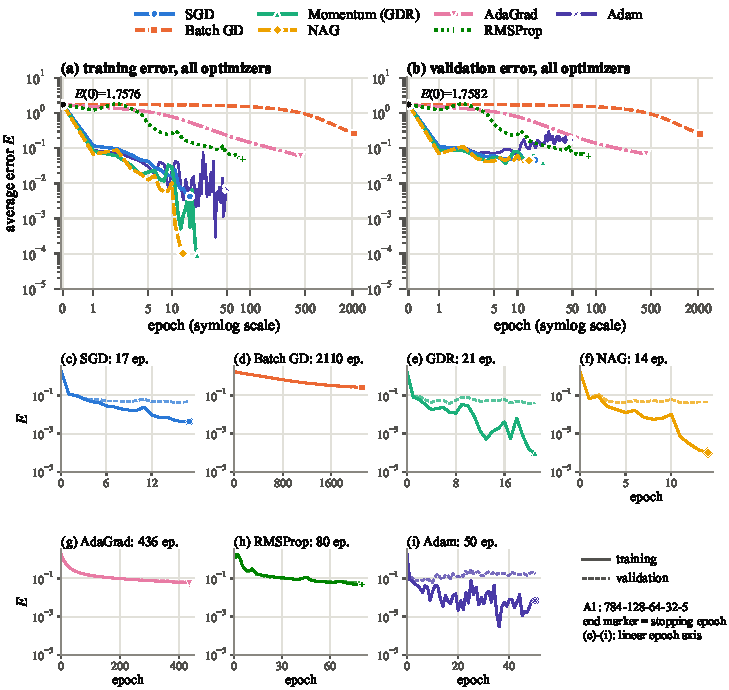
\includegraphics[width=\textwidth]{figures/loss_A1.pdf}
\caption{Training and validation error vs.\ epochs for \textbf{A1} (784--128--64--32--5, wide, 3
hidden layers).}\label{fig:lossA1}
\vspace{3pt}
\begin{minipage}{\textwidth}\small
\textbf{Inference for A1.}
\begin{itemize}
\item NAG is the fastest (14 epochs). GDR reaches the lowest training error ($9.1\times10^{-5}$) and the
best validation accuracy of A1 (99.13\%).
\item GDR also has the lowest validation error of A1, 0.037 at epoch~7. Afterwards it rises slightly
to 0.040, while the training error keeps falling, which is the first sign of over-fitting.
\item SGD and NAG reach their lowest validation error (0.044 and 0.041) close to the stopping epoch.
\item RMSProp (h) has a single spike in which the training error jumps by 0.68. It recovers and
stops after 80 epochs at $E=0.048$.
\item Adam (i) oscillates in 22 epochs. Its validation error grows from 0.062 (epoch 10) to 0.171
although the training error is only 0.007.
\item AdaGrad (g) is perfectly smooth. Its training and validation errors (0.059 and 0.068) fall
together until stopping.
\item Batch GD (d) ends with a validation error (0.251) below its training error (0.263), i.e.\ it
under-fits.
\end{itemize}
\end{minipage}
\end{figure}

\begin{figure}[p]
\centering
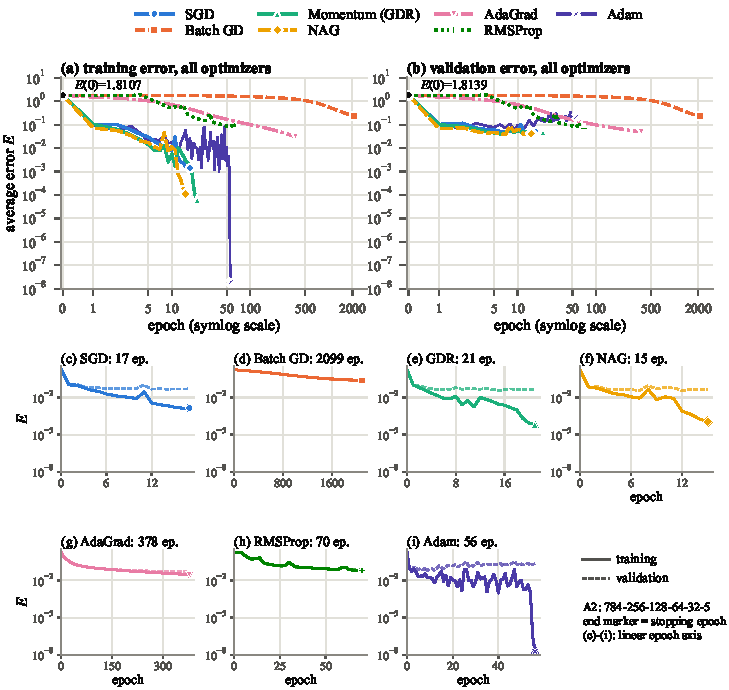
\includegraphics[width=\textwidth]{figures/loss_A2.pdf}
\caption{Training and validation error vs.\ epochs for \textbf{A2} (784--256--128--64--32--5, wide,
4 hidden layers).}\label{fig:lossA2}
\vspace{3pt}
\begin{minipage}{\textwidth}\small
\textbf{Inference for A2.}
\begin{itemize}
\item NAG (f) converges in 15 epochs and reaches the lowest validation error of all 42 runs, 0.037
at epoch 12, together with the highest validation accuracy (99.26\%). This run is the best model.
\item GDR (e) reaches the lowest training error of the momentum methods ($6.2\times10^{-5}$). Its
validation error is lowest at epoch 15 (0.038) and ends at 0.048.
\item Adam (i) shows the typical over-confidence: its training error drops to $1.9\times10^{-8}$ at
epoch 56, while its validation error climbs from 0.061 (epoch 9) to 0.223. This is the largest
training--validation gap of A2.
\item AdaGrad (g) gives the best batch-mode result of the wide networks: $E=0.030$,
$E_{val}=0.049$ and 98.42\% validation accuracy.
\item RMSProp (h) stops after 70 epochs, with its validation error lowest at the stopping epoch (0.069).
\item Batch GD (d) needs 2099 epochs and again under-fits ($E_{val}=0.228<E=0.239$).
\end{itemize}
\end{minipage}
\end{figure}

\begin{figure}[p]
\centering
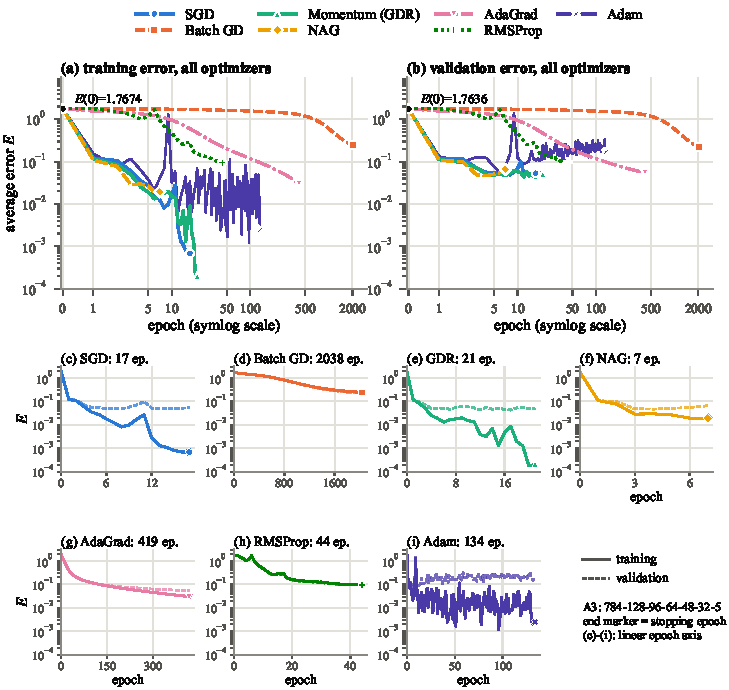
\includegraphics[width=\textwidth]{figures/loss_A3.pdf}
\caption{Training and validation error vs.\ epochs for \textbf{A3} (784--128--96--64--48--32--5,
wide, 5 hidden layers).}\label{fig:lossA3}
\vspace{3pt}
\begin{minipage}{\textwidth}\small
\textbf{Inference for A3.}
\begin{itemize}
\item NAG (f) stops after only 7 epochs on a short plateau ($E=0.0195$). Its validation error had
already risen from 0.047 (epoch 4) to 0.066, so the criterion stopped it at a poor point.
\item SGD and GDR need 17 and 21 epochs and reach training errors of $6.8\times10^{-4}$ and
$2.0\times10^{-4}$.
\item Adam (i) is the most unstable of all runs. Its training error rose in 74 epochs, once by 1.22
within a single epoch, and it needed 134 epochs to stop. Its final weights still give the best
validation accuracy of A3 (99.05\%).
\item RMSProp (h) shows spikes of up to 0.50. It stops after 44 epochs at $E=0.095$ with 96.63\%
validation accuracy, the lowest among the wide networks.
\item AdaGrad (g) decreases monotonically to $E=0.030$.
\item Batch GD (d) under-fits the most: its validation error is 0.020 below its training error.
\end{itemize}
\end{minipage}
\end{figure}

\begin{figure}[p]
\centering
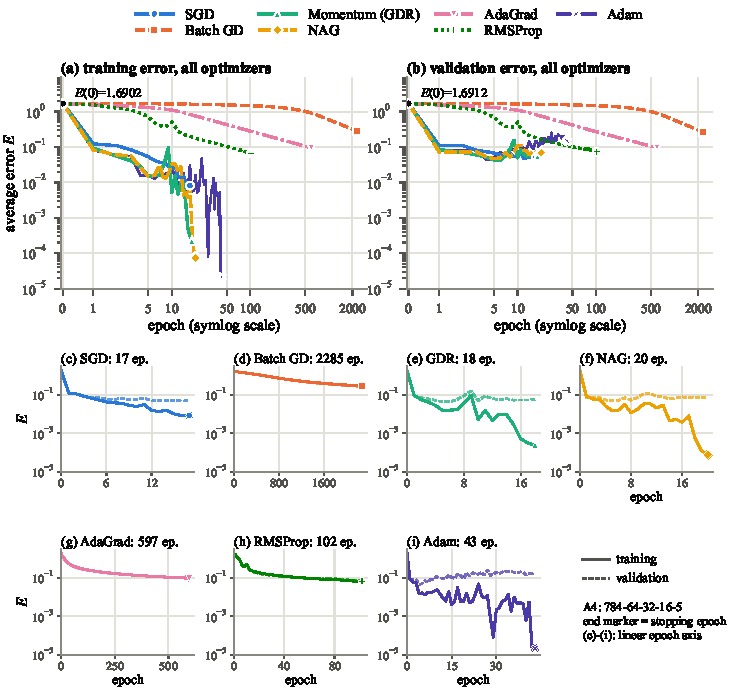
\includegraphics[width=\textwidth]{figures/loss_A4.pdf}
\caption{Training and validation error vs.\ epochs for \textbf{A4} (784--64--32--16--5, narrow, 3
hidden layers).}\label{fig:lossA4}
\vspace{3pt}
\begin{minipage}{\textwidth}\small
\textbf{Inference for A4.}
\begin{itemize}
\item With the fewest parameters (52\,933), SGD (c) stops at the highest SGD error of all networks,
$E=0.0081$.
\item GDR and NAG reach about $10^{-4}$ in 18 and 20 epochs. Their validation error, however, is
lowest early (0.043 at epoch 6 and 0.047 at epoch 5) and then rises by 0.013 and 0.021.
\item Adam (i) is the fastest Adam run (43 epochs). It has the lowest Adam validation error of all
networks (0.044 at epoch 4) and the best validation accuracy of A4 (98.97\%), but its validation error
ends at 0.146.
\item AdaGrad (g) needs 597 epochs and stops at the highest AdaGrad error ($E=0.094$). Its training
and validation errors are almost equal (gap 0.002).
\item RMSProp (h) needs 102 epochs, and its validation error rose in 39 of them.
\item Batch GD (d) stops at $E=0.285$, the highest batch-GD error of all networks.
\end{itemize}
\end{minipage}
\end{figure}

\begin{figure}[p]
\centering
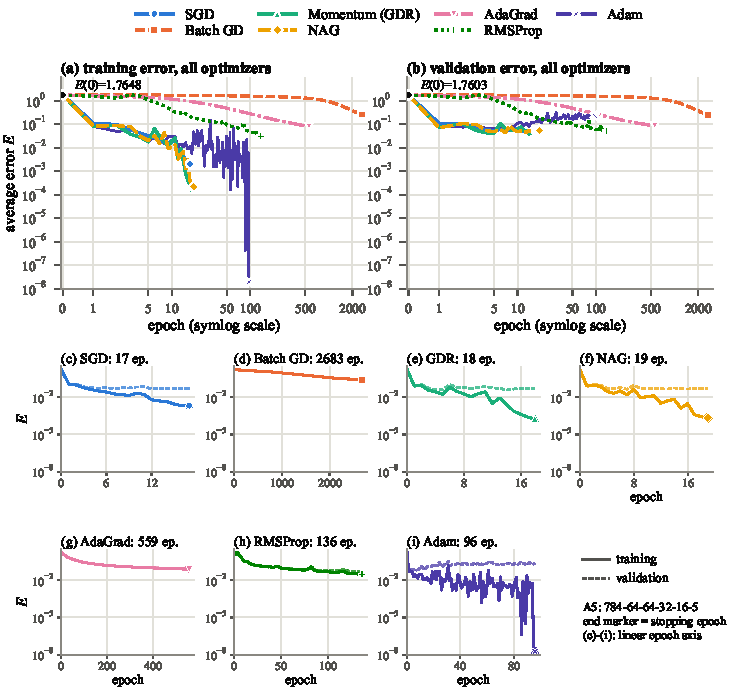
\includegraphics[width=\textwidth]{figures/loss_A5.pdf}
\caption{Training and validation error vs.\ epochs for \textbf{A5} (784--64--64--32--16--5, narrow,
4 hidden layers).}\label{fig:lossA5}
\vspace{3pt}
\begin{minipage}{\textwidth}\small
\textbf{Inference for A5.}
\begin{itemize}
\item Batch GD (d) is the longest run of the whole study (2683 epochs) and stops at $E=0.262$.
\item RMSProp (h) gives its best result on this network: $E=0.031$, $E_{val}=0.052$ and 98.37\%
validation accuracy. Its validation error still rose in 33 epochs, with spikes of up to 0.52.
\item NAG (f) gives the best validation accuracy of A5 (99.00\%). GDR (e) has the lowest validation
error of A5, 0.038 at epoch 14.
\item Adam (i) reaches $E=1.9\times10^{-8}$ after 96 epochs and 46 error rises. Its validation error
grows from 0.065 (epoch 5) to 0.232.
\item AdaGrad (g) needs 559 epochs and stops at $E=0.078$.
\item SGD (c) behaves as on the wide networks (17 epochs, $E=0.0021$).
\end{itemize}
\end{minipage}
\end{figure}

\begin{figure}[p]
\centering
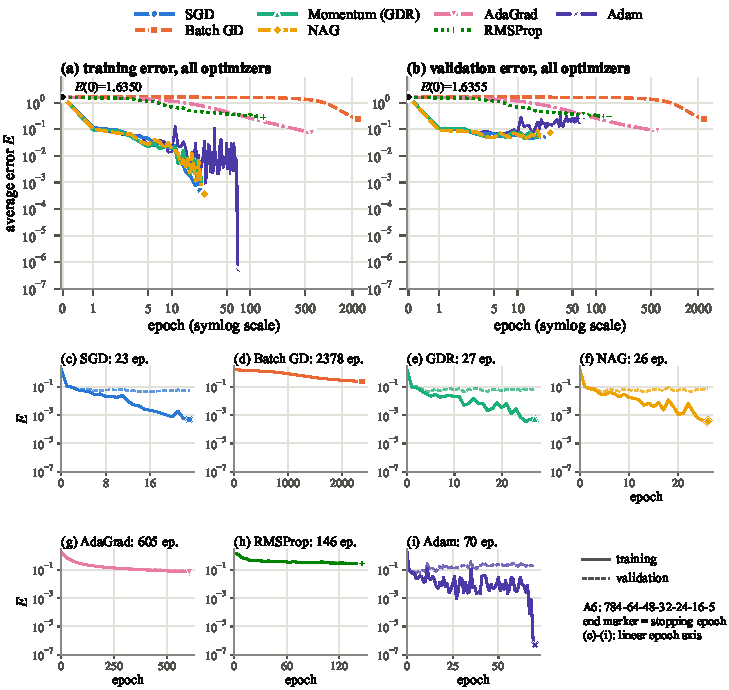
\includegraphics[width=\textwidth]{figures/loss_A6.pdf}
\caption{Training and validation error vs.\ epochs for \textbf{A6} (784--64--48--32--24--16--5,
narrow, 5 hidden layers).}\label{fig:lossA6}
\vspace{3pt}
\begin{minipage}{\textwidth}\small
\textbf{Inference for A6.}
\begin{itemize}
\item On the deepest and narrowest network all pattern-mode optimizers need more epochs than on any
other network: SGD 23, NAG 26 and GDR 27.
\item The validation error of GDR and NAG is lowest at epochs 12--13 (0.047 and 0.044) and then rises
by 0.020 and 0.028, the largest rises of the momentum methods.
\item RMSProp (h) is the weakest run of A6. From epoch 50 on, its error stays between 0.28 and 0.39.
It stopped during a temporary accuracy dip (93.9\% validation accuracy), after its best of 97.8\% at
epoch 105.
\item Adam (i) stops after 70 epochs at $E=4.9\times10^{-7}$. Its validation error grows from 0.067 to
0.251, the largest rise of all Adam runs.
\item AdaGrad (g) needs the most epochs of all AdaGrad runs (605).
\item GDR and NAG share the best validation accuracy of A6 (98.95\%).
\end{itemize}
\end{minipage}
\end{figure}

\FloatBarrier
\subsection{Training and Validation Accuracy}
Table~\ref{tab:acc} reports the training and validation accuracy of the weights at the stopping
epoch for every optimizer and architecture.

\begin{table}[!htb]
\centering
\caption{Training and validation accuracy (\%) at convergence. The best validation accuracy of each
architecture is shown in bold, and the overall best (A2 with NAG) is also underlined.}\label{tab:acc}
\setlength{\tabcolsep}{4.6pt}
\begin{tabular}{llrrrrrrr}
\toprule
Arch. & Set & SGD & BGD & GDR & NAG & AdaGrad & RMSProp & Adam \\
 & & {\scriptsize $B{=}1$} & {\scriptsize $B{=}N$} & {\scriptsize $B{=}1$} & {\scriptsize $B{=}1$} & {\scriptsize $B{=}N$} & {\scriptsize $B{=}N$} & {\scriptsize $B{=}1$} \\
\midrule
A1 & Train & 99.96 & 93.54 & 100.00 & 100.00 & 98.45 & 98.65 & 99.96 \\
 & Val & 98.45 & 94.26 & \textbf{99.13} & 98.97 & 97.79 & 97.92 & 99.03 \\
\addlinespace[2pt]
A2 & Train & 99.99 & 94.05 & 100.00 & 100.00 & 99.41 & 98.11 & 100.00 \\
 & Val & 98.68 & 94.47 & 99.05 & \underline{\textbf{99.26}} & 98.42 & 97.84 & 98.87 \\
\addlinespace[2pt]
A3 & Train & 100.00 & 93.50 & 99.99 & 99.44 & 99.32 & 97.20 & 99.97 \\
 & Val & 98.55 & 94.60 & 98.95 & 98.39 & 98.34 & 96.63 & \textbf{99.05} \\
\addlinespace[2pt]
A4 & Train & 99.91 & 92.94 & 100.00 & 100.00 & 97.66 & 98.08 & 100.00 \\
 & Val & 98.52 & 93.94 & 98.95 & 98.84 & 97.47 & 97.73 & \textbf{98.97} \\
\addlinespace[2pt]
A5 & Train & 99.99 & 93.77 & 100.00 & 99.99 & 97.95 & 99.18 & 100.00 \\
 & Val & 98.63 & 93.97 & 98.92 & \textbf{99.00} & 97.60 & 98.37 & 98.66 \\
\addlinespace[2pt]
A6 & Train & 100.00 & 93.47 & 100.00 & 99.98 & 98.22 & 94.60 & 100.00 \\
 & Val & 98.68 & 93.81 & \textbf{98.95} & \textbf{98.95} & 97.58 & 93.89 & 98.66 \\
\bottomrule
\end{tabular}

\end{table}

\Needspace{6\baselineskip}
\paragraph{Observations.}
\begin{itemize}
\item \textbf{The optimizer matters more than the architecture.} SGD, GDR, NAG and Adam fit the
training set almost perfectly (99.4--100\%) and reach 98.4--99.3\% validation accuracy. AdaGrad
reaches 97.5--98.4\%, RMSProp 93.9--98.4\% and batch GD only 93.8--94.6\%.
\item \textbf{Width helps a little, depth does not.} The best validation accuracies are 99.13\%,
99.26\% and 99.05\% for the wide networks A1--A3 and 98.97\%, 99.00\% and 98.95\% for the narrow
networks A4--A6. For every depth the wide network is 0.1--0.3 percentage points better. In both
families the network with four hidden layers is best, so more depth alone does not help.
\item \textbf{Generalisation.} The pattern-mode optimizers show a small gap of 0.7--1.5 percentage
points between training and validation accuracy, i.e.\ mild over-fitting. Batch GD is the only
optimizer whose validation accuracy exceeds its training accuracy (under-fitting).
\end{itemize}

\subsection{Best Architecture}
The highest validation accuracy of all 42 runs, 99.26\%, is obtained by architecture \textbf{A2}
(784--256--128--64--32--5) trained with \textbf{NAG}, which converged in 15 epochs. It is therefore
chosen as the best model. Figure~\ref{fig:cm} shows its training and test confusion matrices.

\begin{figure}[!htb]
\centering
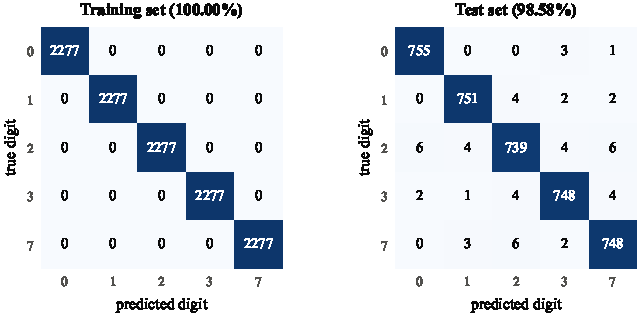
\includegraphics[width=0.8\textwidth]{figures/confusion_best.pdf}
\caption{Confusion matrices of the best model (A2 trained with NAG) on the training set (left) and the
test set (right). The accuracy is given in the title and cell shading shows the row-normalised rate.}\label{fig:cm}
\vspace{2pt}
\begin{minipage}{\textwidth}\small
\textbf{Inference.} All 11\,385 training images are classified correctly (100.00\%) and 3741 of the
3795 test images (\textbf{test accuracy 98.58\%}), 0.7 percentage points below the validation
accuracy. Digit~2 is the hardest class (20 of 759 test images wrong, mostly predicted as 0 or 7).
Digits 0 and 1 are recognised best (755 and 751 correct).
\end{minipage}
\end{figure}

\FloatBarrier
\section{Conclusion}
Seven optimizers for back-propagation were compared on six FCNNs, a wide and a narrow network with
three, four and five hidden layers each. All runs used identical conditions: the same initial
weights, data order, error function, learning rate and stopping rule, with every update rule
implemented exactly as in the course material. Pattern-mode training with momentum gives the best
trade-off. NAG and the generalised delta rule converge within 7--27 epochs, and NAG yields the best
model, A2 with 99.26\% validation and 98.58\% test accuracy. Vanilla batch gradient descent with
$\eta=0.001$ is impractically slow and under-fits. AdaGrad and RMSProp make batch-mode training 4--46
times faster in epochs, but with one update per epoch they stop at a higher error. Adam reaches the
lowest training errors but is noisy with a batch size of one and becomes over-confident, so its
validation error rises. Wide networks are slightly more accurate than narrow ones, while depths from
three to five hidden layers perform similarly. Finally, the criterion
$|E(t)-E(t-1)|<10^{-4}$ detects a lack of progress rather than optimality. It can stop runs that are
merely slow (batch GD, AdaGrad) or at a turning point of a noisy curve (RMSProp, NAG on A3), and the
validation error of the pattern-mode optimizers is lowest well before stopping. It should therefore
be used together with validation monitoring.

\begin{thebibliography}{8}
\bibitem{rumelhart1986}
Rumelhart, D.E., Hinton, G.E., Williams, R.J.: Learning representations by back-propagating
errors. Nature \textbf{323}, 533--536 (1986)

\bibitem{nesterov1983}
Nesterov, Y.: A method for solving the convex programming problem with convergence rate
$O(1/k^2)$. Soviet Mathematics Doklady \textbf{27}, 372--376 (1983)

\bibitem{duchi2011}
Duchi, J., Hazan, E., Singer, Y.: Adaptive subgradient methods for online learning and stochastic
optimization. Journal of Machine Learning Research \textbf{12}, 2121--2159 (2011)

\bibitem{tieleman2012}
Tieleman, T., Hinton, G.: Lecture 6.5 -- RMSProp: Divide the gradient by a running average of its
recent magnitude. COURSERA: Neural Networks for Machine Learning (2012)

\bibitem{kingma2015}
Kingma, D.P., Ba, J.: Adam: A method for stochastic optimization. In: 3rd International Conference
on Learning Representations (ICLR) (2015)

\bibitem{kumar2013}
Kumar, S.: Neural Networks -- A Classroom Approach, 2nd edn. Tata McGraw-Hill (2013)

\bibitem{aggarwal2018}
Aggarwal, C.C.: Neural Networks and Deep Learning. Springer (2018)

\bibitem{he2015}
He, K., Zhang, X., Ren, S., Sun, J.: Delving deep into rectifiers: Surpassing human-level
performance on ImageNet classification. In: IEEE International Conference on Computer Vision
(ICCV), pp. 1026--1034 (2015)
\end{thebibliography}

\end{document}
